%
% Based on Simple CV template by Sofia JIJON
% https://github.com/sjijon/TeX-templates
%

\documentclass[a4paper,10pt]{article}

% Packages
\usepackage[vmargin=1cm, hmargin=1cm]{geometry}
\usepackage[latin1]{inputenc}
\usepackage[T1]{fontenc}
\usepackage[english]{babel}
\usepackage{fontawesome}
\usepackage{datetime}
\usepackage[colorlinks=true, urlcolor=ColorTwo]{hyperref}
\usepackage{tikz}
\usepackage{enumitem}
\usepackage{sectsty}
\usepackage{multicol}
\usepackage{adjustbox}

% Color theme
\definecolor{ColorOne}{RGB}{0,110,140} 	% Blue
\definecolor{ColorTwo}{RGB}{120,0,120} 	% Mauve
%\definecolor{ColorTwo}{RGB}{140,100,0} % Gold

\sectionfont{\color{ColorOne}} 
\subsectionfont{\color{ColorOne}} 

% Pretty C++
\def\CC{{C\nolinebreak[4]\hspace{-.05em}\raisebox{.4ex}{\tiny\bf ++}}}

%--------------------------------------------------------------------------------------------------------------

\begin{document}
\thispagestyle{empty}

%--------------------------------------------------------------------------------------------------------------
% Left column begin
%--------------------------------------------------------------------------------------------------------------
\begin{adjustbox}{valign=t}
\begin{minipage}{0.3\textwidth} % width

% Photo
\begin{center}
\begin{tikzpicture}
	\clip (0,0) circle (2cm) node {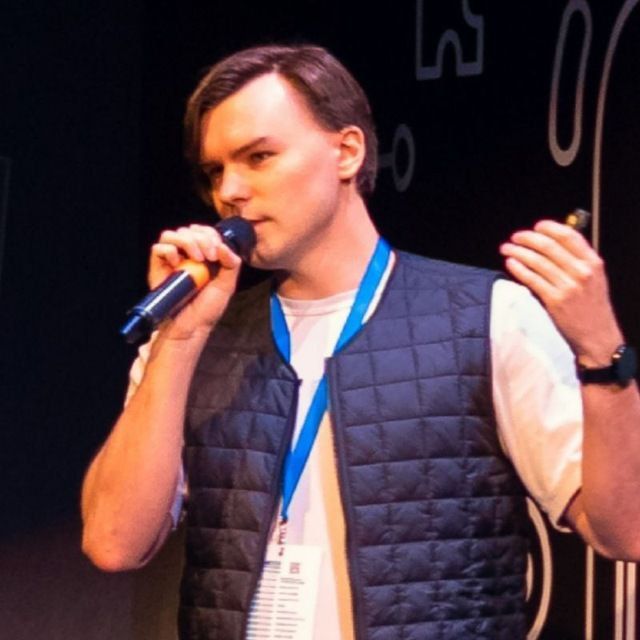
\includegraphics[width=4cm]{../img/1.jpeg}};
\end{tikzpicture}
\vspace{10 pt}

% Name
{\LARGE \bfseries Danil Neverov}\\
\vspace{10 pt}
Currently in\\
Saint Petersburg, Russia

% Links
\textcolor{ColorTwo}{\faEnvelopeO} 
\href{mailto:danil.nev@gmail.com}{danil.nev@gmail.com} \\
\textcolor{ColorTwo}{\faChain} 
\href{https://www.linkedin.com/in/danil-neverov-37567066/}{LinkedIn}
%\textcolor{ColorTwo}{\faChain} 
%\myhref{https://github.com/SayHey}{GitHub}
\end{center}
\vfill

% Professional Skills Section----------------------------------------------------------------------------------
\section*{Professional Skills}
\raggedright
\begin{enumerate}[align = left, labelwidth = 4em, leftmargin = \dimexpr\labelwidth + \labelsep\relax]
	\item [\textcolor{ColorOne}{$\bullet \bullet \bullet \, \bullet $}] \CC, Applied Math
	\item [\textcolor{ColorOne}{$\bullet \bullet \bullet \, \circ $}] Linux, CMake, Git, CI/CD, Team Management
	\item [\textcolor{ColorOne}{$\bullet \bullet \circ \, \circ $}] Python, Matlab
	\item [\textcolor{ColorOne}{$\bullet \circ \circ \, \circ $}] CAM/G-Code, \\CAD Modeling, \\PLC Programming
\end{enumerate}
\vfill

% Education Section--------------------------------------------------------------------------------------------
\section*{Education}
\raggedright
\textcolor{ColorOne}{2013.}
\textbf{Saint Petersburg State University}\\
Specialist degree in Applied Mathematics and Computer Science\\
\textit{GPA 4.8/5 Diploma with distinction}
\vspace{10 pt}

\textcolor{ColorOne}{2008.}
\textbf{Fadeeev Academic Gymnasium of SPSU}\\

	
% Update time
\vspace{240 pt}
\centering \small
\textcolor{ColorOne}{Last updated: \monthname,~\the\year.}

\end{minipage}
\end{adjustbox}
%--------------------------------------------------------------------------------------------------------------
% Left column end
%--------------------------------------------------------------------------------------------------------------
%
% Vertical rule------------------------------------------------------------------------------------------------
\hfill
\begin{adjustbox}{valign=t}
\begin{minipage}{0.05\textwidth} % width
\textcolor{ColorOne}{\rule{1pt}{\textheight}}
\end{minipage}
\end{adjustbox}
\hfill
%
%--------------------------------------------------------------------------------------------------------------
% Right column begin
%--------------------------------------------------------------------------------------------------------------
\begin{adjustbox}{valign=t}
\begin{minipage}{0.6\textwidth} % width

% Professional Experience Section------------------------------------------------------------------------------
\section*{Professional Experience}
\raggedright
\textcolor{ColorOne}{Aug. 2018 -- Aug. 2022}\\
\emph{\textbf{Tech Lead of Robot Driver team}} at \textbf{ARRIVAL}\\
London, UK / Saint Petersburg, Russia\\
\vspace{10 pt}
The main focus of our department was the software platform for the flexible fully autonomous robotic factory.
I started as a developer and later became a team lead of 7 developers. We covered a hardware interaction layer 
of this platform. That includes polymorphic vendor- agnostic hardware communication, as well as custom real-time
feedback controllers for specific robotic operations, which involved CV feedback, force feedback and direct 
torque/current control of robot motors. We called it Robot Driver. It runs on edge devices with Linux Preempt RT.
My responsibilities included:
\begin{itemize}[noitemsep]
	\item Designing and implementing various feedback controllers and robot motion features on modern \CC 
	(up to \CC20);
	\item Developing the architecture for a realtime Linux-based software that wraps these features as well as 
	hardware communication and higher level MES communication into a single product;
	\item Analyzing data from sensors and metrological systems;
	\item Managing tasks for the team, enforcing good software practices, maintaining the long term product vision
	and roadmap;
	\item Communicating with other teams, higher management and external partners (contractors, universities, etc),
	presenting for the internal and external demos (investors, universities, etc.).
\end{itemize}
Information: \href{https://arrival.com}{\underline{arrival.com}}
\vspace{10 pt}
	
\textcolor{ColorOne}{Aug. 2013 -- Aug. 2018}\\
\emph{\textbf{\CC Developer - Mathematician}} at \textbf{CIMCO Software}\\
Copenhagen, Denmark / Saint Petersburg, Russia\\
\vspace{10 pt}
Developed a mathematical core for CAD/CAM software:
\begin{itemize}
	\item Worked on the new project of CNC toolpath generation software. My work consisted of designing complex 
		computational geometry algorithms and implementing them using \CC. I have done several 3-axis milling 
		strategies, including some unique cutting edge strategies that didn't exist before. \\
		Information: 
		\href{https://www.mastercam.dk/hsm-performance-pack/product/machining-strategies}
		{\underline{mastercam.dk/hsm-performance-pack/}}
	\item Supported and expanded the functionality of 2D CAD editor. Developed a geometric 
		library for working with 2D primitives.\\
		Information: 
		\href{https://www.cimco.com/software/cimco-cnc-calc}
		{\underline{cimco.com/software/cimco-cnc-calc}}
\end{itemize}

% Personal Section---------------------------------------------------------------------------------------------
\section*{Personal}
\begin{itemize}[noitemsep]
	\item I am an active enthusiast of DIY culture. I assembled and programmed two quadcopters out of hobby parts 
		and Arduino.
	\item I occasionally participate in various hackatons and competitions such as TrackML. Back in school and 
		university I won several local and state math and physical competitions among students.
	\item I am always eager to learn more so I am an active user of various online educational resources as well 
		as offline seminars and meetings. I also occasionally participate in such events as a speaker.
	\item My scientific and professional areas of interest, in which I did my personal projects and 
		maintain educational efforts are the following:
	\begin{itemize}[noitemsep]
        \item Industrial automation, Robotics, ML, Artificial Intelligence
        \item Computer-Aided everything including CAD, CAM and 
		\item Computer-Aided Biotechnology, Bioinformatics, Neurosciences
		\item Quantum Computing, Theoretical Physics and Math
	\end{itemize}
	\item As for non-professionally related activities and interests 
	I like Snow/Surf/Skateboarding, MTB, Japanese cars and Esports.
\end{itemize}

\end{minipage}
\end{adjustbox}
%--------------------------------------------------------------------------------------------------------------
% Right column begin
%--------------------------------------------------------------------------------------------------------------
\end{document}
